\subsection{Model design (Jens Carl)}
% Main classes: User, Customer, Admin, Account
% Wrapper-ish: TransactionHistoryElement, Valuta
%
% Points:
% We looked at existing net banking applications
% and used them as inspiration. 
% We also used our own experience and intuition
% to build the data model.
% 
% Starting with an idea of logging in as an user % through a webapplication helped us grasp the 
% problem domain and get a good starting point.
%
% From there on the model began forming itself
% - It became evident that out vision of being 
%   a user was split into two parts: customer and
%   admins. 
% - A user is an abstract entitiy that can either %   take shape as an admin or as a customer.
% - 
%Starting with an idea of logging in as an user through a webapplication helped us 

%we wanted the data model to mimic the beheavior of the subject at hand: the user of the application. Therefore we want an abstract entity 'User' which can take form as either a 'Customer' or an administrator 'Admin' logging on. 
%The person using the application (e.g. user).Wether this user is a customer of the bank, or an intern working as an administrator (e.g. admin). His/Hers potential accounts. And last, but not least, other users and accounts \begin{itemize}
%    \item The person using the application %(e.g. user).
%    \item Wether this user is a customer of the bank, or an intern working as an administrator (e.g. admin).
%    \item His/Hers potential accounts.
%\end{itemize}to interact with.
%\begin{itemize}
%    \item[--] Users; members of the bank. Core information about users must be stored in the database. This includes login credentials (username, password) and a name.
%    \item[--] Customers. If a user is a customer, linkage to his/hers account(s) must also be stored, along with customer-unique preferences. 
%    \item[--] Admins. If a user is an administrator, working at the bank, his/hers    
%    \end{itemize}
% Designing on an object-oriented basis, we took key elements in the problem domain and devided them into objects:
% \begin{itemize}
%     \item[--] Users; members of the bank. Core information about users must be stored in the database. This includes login credentials (username, password) and a name. There are two kinds of users:
%     \begin{itemize}
%         \item[--] Customers; possesing accounts and unique preferences. 
%         \item[--] Admins; no extra data other than the type. 
%     \end{itemize} 
%     \item[--] Accounts; 
% \end{itemize}
%Thus, our model takes its starting point in the thought of frequent fetching/storing from/to a database.

%introduction
The database was an essential part of the model component of MVC. It provides the ability to store information between sessions, which can be accessed by computers with a connection. For an online banking application, this is exactly what's needed. 

When designing the table structure of the database, we mirrored elements in the problem domain: We wanted customers, accounts and admins to be the core entities in the application, so we made tables for those. See figure \ref{fig:wackyModelDesign}.
\begin{figure}[!htb]
    \centering
    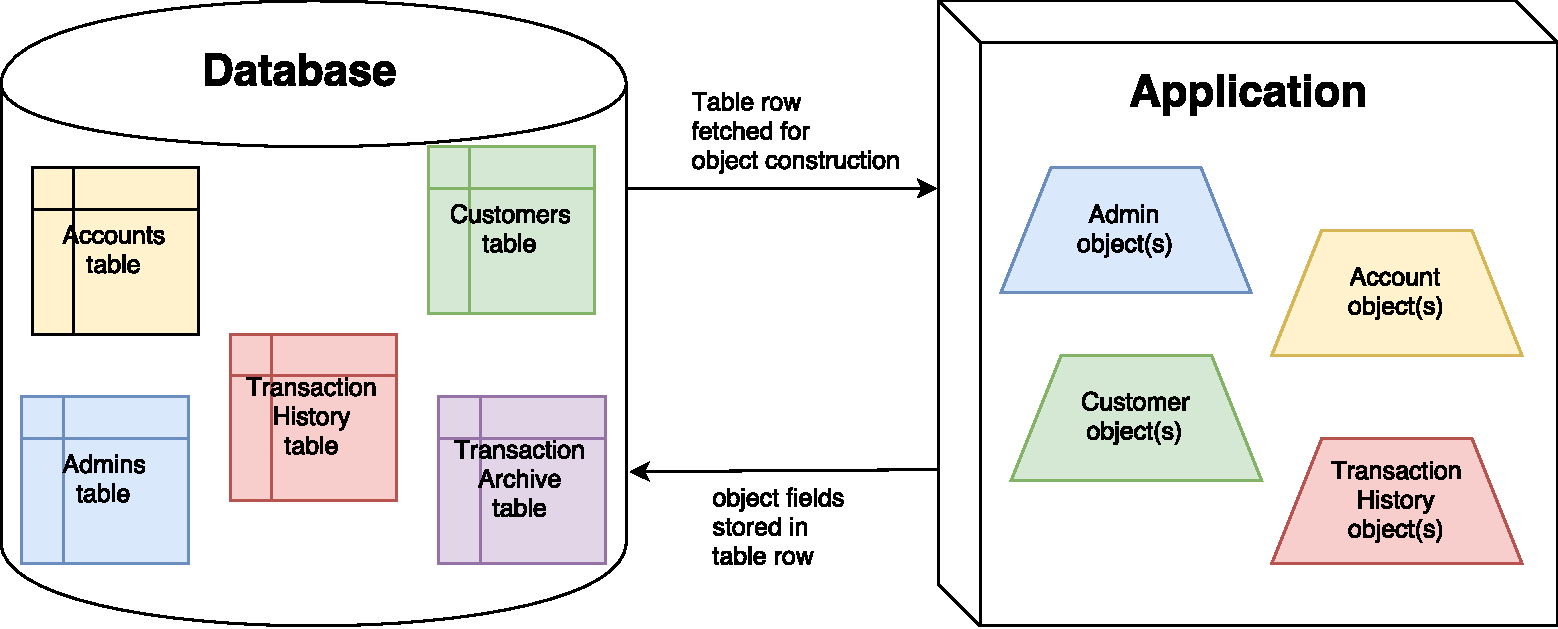
\includegraphics[scale=.5]{figures/modelDesign.pdf}
    \caption{Figure illustrating how the model is designed with the database in mind. Designing on an object-oriented basis, we took key elements in the problem domain and divided them into sections. There are 'Customers' of the bank with  bank 'Accounts'. Their transactions are stored in the 
    'Transaction History'. Lastly there are also 'Admins' working at the bank, with special privileges.}
    \label{fig:wackyModelDesign}
\end{figure} 

In the application, the model is almost mirrored the database, except that instead of storing \textit{every} customer, only a few relevant are stored locally each session of use. Objects are constructed with the information provided in a given row of the tables, and they're modified during the session of user interaction. When changes are committed, the data in the same objects are stored in their corresponding table rows.